\section{Overview}
\label{sec:overview}

\subsection{\xxx Work Flow}

\xxx operates in two phases.  A user runs command ``\v{\xxx start}'' to
enter the system-wide tracing phase, within which \xxx logs events
including system calls, inter-process communications (IPCs), and waits and
wake-ups from all applications and daemons.  Occasionally based on user
configurations, it logs data flag accesses leveraging hardware
watch-point registers.  Each log entry includes a timestamp, the event
type, key attributes of the event, and a lightweight call stack obtained
by unwinding the stack pointer.  \xxx implements tracing by instrumenting
core system libraries and a small portion of the operating system.  The
performance impact of this system-wide tracing is low because the logged
events themselves are often expensive and require user-kernel crossings,
masking the overhead of tracing.

Whenever a user detects a performance issue such as a spinning cursor, she
runs ``\v{\xxx debug}'' to enter the interactive diagnosis phase.  \xxx
initializes this phase by constructing a causal graph from all logged
events up to user-specified duration.  Rather than requiring a precise
application-specific user-written schema, \xxx leverages a simple
system-wide schema we created to construct approximate graphs
(\S\ref{subsec:graph}), and relies on interactive user insights for
diagnosis (\S\ref{subsec:debug}).

\subsubsection{Constructing Event Graphs} \label{subsec:graph}

\xxx defines the beginning of an execution segment as one of the following
three types of events (1) the beginning of a thread, (2) the event from a
wait operation such as \v{pthread\_cond\_wait()} or
\v{mach\_msg\_receive()}, and (3) the first logged event of a thread
because tracing may start mid execution.  It similarly defines the end of
an execution segment as (1) the exit of a thread, (2) the call to a wait
operation, and (3) the last logged event of a thread.

\xxx defines the edges as follows.  First, the return from a wait
operation causally depends on the wake-up operation.  Since an application
or its libraries may define custom synchronization primitives, \xxx traces
wait and wake-up operations inside the operating system kernel (the
\v{mach\_os\_wait} and \v{mac\_os\_signal} XXX functions in MacOS kernel).
This design decision ensures that \xxx captures a large set of casual
edges at the expense of superfluous edges that do not map to causality.
For instance, inside a system call or interrupt handler, the kernel
typically checks whether the current process has used up its time slice
and, if so, wakes up another process.  \xxx thus explicitly filters out
edges due to kernel maintenance (in \v{mac\_os\_interrupt()} and
\v{timeshare\_maintenance in MacOS}) instead of application intent.
Second, the read of a data flag causally depends on the write of the
same flag.  Edges of this type are few but critical for diagnosis.  Third,
the timer expiration and cancellation events causally depend on the
installation of the timer.  Fourth, each execution segment has an incoming
edge from the immediately preceding segment in the same thread.  \xxx
considers this type of intra-thread edges weaker than inter-thread edges
due to the wait between the two segments.  In its analysis, \xxx follows
intra-thread edges typically only when it cannot find any inter-thread
edges.

It is easy for a user to incrementally extend \xxx with custom segment
boundaries and edges.  For instance, to handle batch processing, we
created a heuristic that splits a segment if it has outgoing edges to two
or more different processes (unless the attributes of the corresponding
events indicate otherwise).  We also added edges for three data flags and
XXX custom communication primitives (see \S\ref{xxx}).

\subsubsection{Interactive Diagnosis} \label{subsec:debug}

After \xxx builds the event graph, a user can interactively query this
graph for diagnosis.  For instance, consider a spinning cursor in MacOS
which indicates the current application's main thread has not processed
any UI events for over two seconds.  The user can query \xxx to find the
ongoing event in the application's main thread concurrent to the display
of the spinning cursor.  Depending on the type of the event, she can
proceed in three directions.

First, if the concurrent event is a busy operation that occupies the CPU,
she has found the cause of the spinning because a busy main thread cannot
process UI events.  She can examine the event's lightweight call stack.
If it does not provide enough details, she can rerun the application and
use \xxx's fine-grained debugging tool to obtain a more complete call
stack, the addresses of the instructions executed, and parameters and
return values of call instructions.  In general, she can increase
debugging details for any event, not just a busy event.

Second, if the concurrent event is a blocking wait, she runs \xxx to
locate another event in the graph that causes the wake-up to arrive
late. \xxx does so using the following idea.  In the normal case, there
must be a path of wake-up edges that leads to the blocking wait, so the
main thread starts running again.  In the spinning case, somewhere along
the path, a thread's wake-up is missing, so this thread is the culprit.
Mechanically, \xxx first searches the graph to find a similar wait that
does not cause a spinning cursor.  If there are multiple nodes similar to
the wait, \xxx asks the user to pick one.  It then slices the graph
backwards to find the wake-up path.  If an event has exactly one
inter-thread edge or only an intra-thread edge, it follows the edge.
Otherwise, the event must have two or more inter-thread edges, and \xxx
consults the user to pick one to follow.  Given the path, \xxx examples
the threads in the path one by one, and returns the thread whose wake-up
is missing in the spinning case.

Third, if the concurrent event is a thread yield, it is highly indicative
that the main thread is waiting on a data flag (\eg, ``while(!done)
thread\_switch();'').  To discover a data flag, the user reruns the
application with \xxx to collect instruction traces of the concurrent
event in both the normal and spinning cases and detects where the control
flow diverges.  She then reruns the application with \xxx to collect
register values for the basic blocks before the divergence and uncovers
the address of the data flag.  She then configures \xxx to log accesses to
the flag during system-wide tracing.

The user can recursively apply \xxx to further diagnose ``the culprit of
the culprit.''  For instance, 

Based on our results, the first type of spinning cursor is more common but
the second and third types cause the most harm.  The reason is that the
first type tends to be straightforward to diagnose, so they are fixed
quickly.  The second and third types involve multiple threads, so they are
extremely hard to understand and fix even for the application's own
developers.  Therefore, they remain open for years and ruin many users'
experiences.


\subsection{Example: The Chromium Spinning Cursor}

%   resolve symbol, save to log
%     search for set\_spinning
%     if found,
%       find main thread node at the time of set\_spinning
%     find fontd
%     manually check nodes in each thread immediately after the nodes in the slice (normal abnormal boundary)
%  output is a node, and a HTML dump of node and immediate predecessors and successors
% systems preference          
%  spinning node in UI thread is not waiting
%  so we look for messages, and find the diff

Our \xxx prototype is designed to debug performance issues in complex modern applications.
It performs lightweight full system tracing of every process including system calls,
interprocess messages, and MacOS system daemons.
Offline, we build a graph based on thread executions, with nodes defined by
per-request execution segments,
and edges wherever there are temporal constraints between threads of execution.

Upon the graph, we build a set of tools to:
a) inspect the graph,
b) perform slicing on the graph to show dependent nodes,
c) compare graph slices between normal and spinning cases, and
d) select a graph node to gather more information with our debugger scripts.

\begin{figure*}[tb]
    \centering
    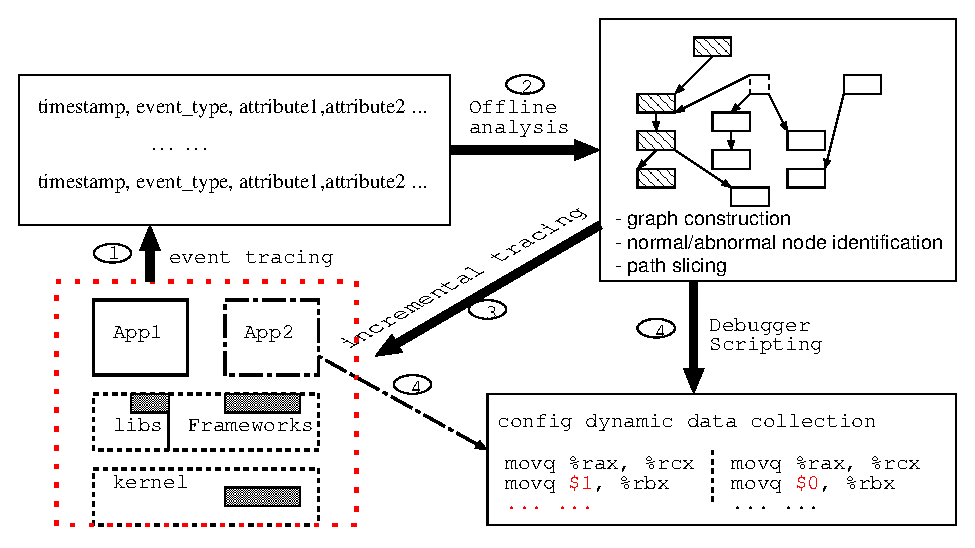
\includegraphics[width=0.7\linewidth]{ArgusOverview.eps}
    \caption{Design Overview}
    \label{fig:argus-overview}
\end{figure*}

For a simple issue, like a rare segmentation fault,
just having lightweight logs may be enough to perform a diagnosis.
However, in most cases, user need to be able to reproduce and gathering
additional data to debug the affected application.
\xxx, shown in Figure \ref{fig:argus-overview} helps the users in the way
it 1) records the system activity 24X7 to capture the reappearance of the bugs,
2) provides tools for the users to gathering more detailed logs,
3) allows users' interactions in the pathing finding,
leaveraging human's superior pattern recognition ability.

We show the general process of interactive debugging using \xxx,
as is shown in Figure\ref{fig:argus-overview},
on Chromium bug in the remaining of the section.

Occasionally when users type non-English characters to search box in Chromium,
the browser get frozen with the spinning cursor.
By attaching the lldb to the main thread of browser, it is not hard to tell that
the main thread blocks on the method \textit{TextInputClientMac::GetFirstRectForRange},
invoking a synchronous IPC to a renderer process.
Although developers knew there was a deadlock between the browser and the renderer,
they did not know how the daedlock occured in the real-world.


\subsection{Event Tracing}

\xxx can continuously run live in the background and collect logs,
leveraging the event tracing infrastructure builtin the system.
The user works as usual until a performance issue is observed.
A log contains a stream of timestamped events with the following format:

\textit{timestamp, Mach\_IPC\_msg\_send, ...}

An event consists of a timestamp, an event type name to annotate current activity,
and arbitrary attributes.
We augment the existing event types with more attributes to support our extensive usage.
For exmaple, we suprisingly found that few traditional RPC style messages presented in the system.
The XPC between SCIM to Chromium spans over four threads.
$SCIM_{tid1}$ sent message and the message was received by $Chromium_{tid1}$.
The reply message was sent from $Chromium_{tid2}$ and received by $SCIM_{tid2}$.
We augment the attributes of Mach\_IPC\_msg with the port information from the messge header.
We also add new types of tracing events when necessary in kernel and libraries.

The log collects the tracing event both in 
a) a baseline situation where the program runs normally,
and b) a spinning situation that exposes the performance issue.
It saved for offline analysis.

\subsection{Offline Graph Construction}
Smilar to traditional causual tracing,
\xxx converts the log into relationship graphs,
by two steps:
linking events reflects correlations system-wide, 
and decomplexing different request segments in the same thread.
The rules are defined as event schema.

Compared to Magpie which requires user input event schema,
\xxx defines event schema initially in the system,
which coveres mostly required event types and rules
for graph construction.
\xxx began graph generation from the event schema
that traditional causual tracing used,
listed in\ref{subsec:traditional event schema},
and corrected them by inspecting the violation patterns in the graph.

\begin{figure*}[tb]
    \centering
    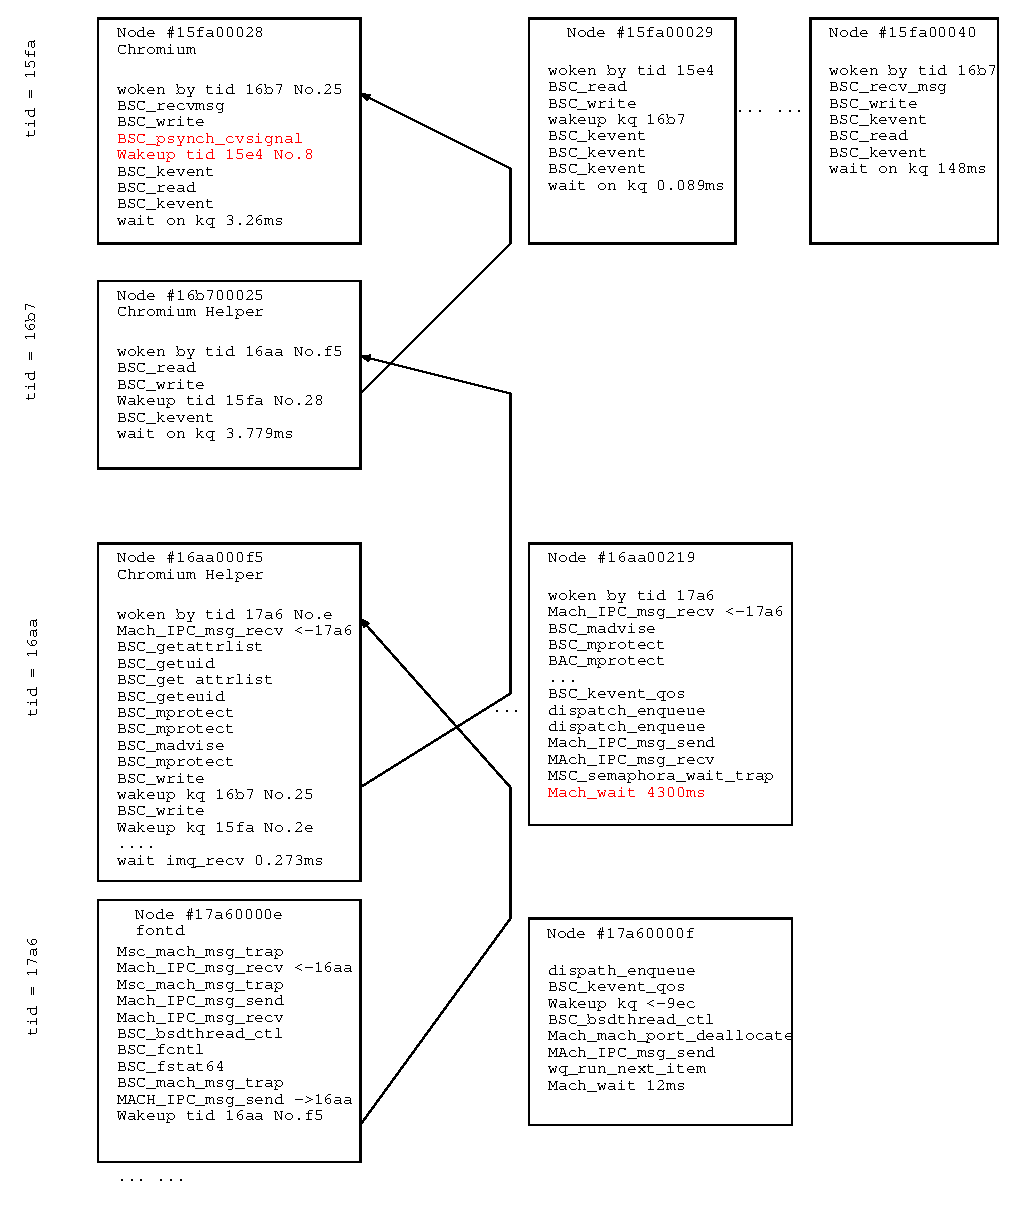
\includegraphics[width=0.9\linewidth]{backward_slicing_chromium.eps}
    \caption{Chromium backward path slicing.}
    \label{fig:path-slice-on-chromium}
\end{figure*}

\begin{figure}[tb]
    \centering
    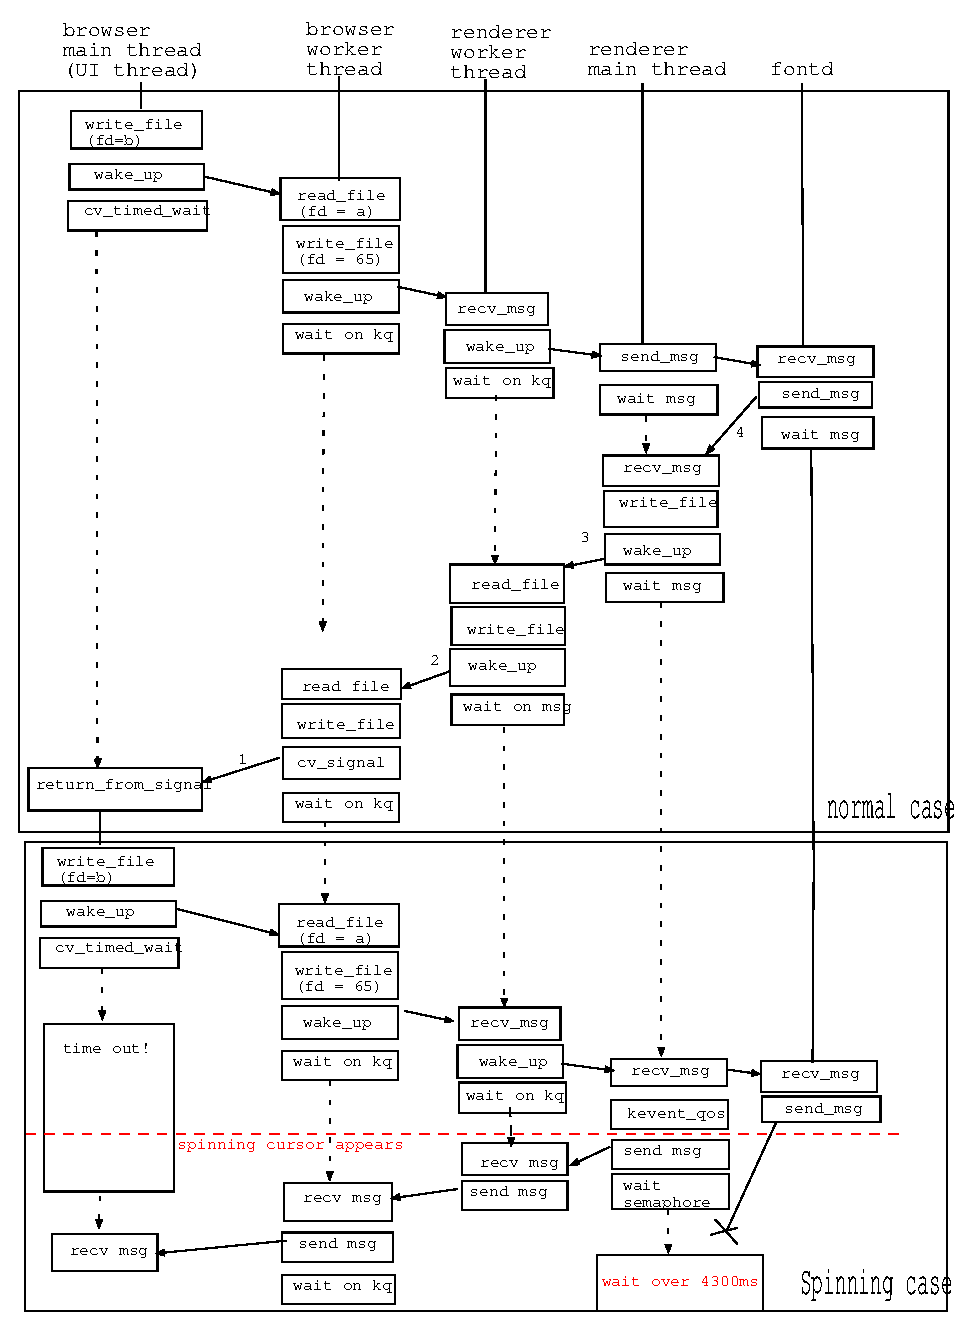
\includegraphics[width=1.0\linewidth]{chromium_case_study.eps}
    \caption{Chromium case study.}
    \label{fig:chromium-trace}
\end{figure}

Traditional causal tracing usually assume one task from
the task queue works on behalf of a request.
However, in MacOS the dequeue block can act as an server,
to process requests from different applications.
As is the nodes \textit{Node\#17a60000c} shown in Figure\ref{fig:path-slice-on-chromium},
fontd dequeues a block and invokes \textit{dispatch\_mig\_server}
in the block to processing message from
different processes.
\begin{lstlisting}[basicstyle=\small\linespread{0.6}]
block = dispatch_queue.dequeue()
dispatch_execute(block)
{
  dispatch_mig_server()
}

dispatch_msg_server()
{
  for(;;) {
    mach_msg(send_reply, recev_request)
    call_back()
    set_reply()
  }
}
\end{lstlisting}

The synchronization between two threads does not
always indicate the causality.
As is shown in \textit{Node\#17a60000d}, the kernel takes over the fontd's thread context to process
interrupts, and wakeup a kernel thread.
As a result, to generate a more concise relationship graph,
we defined additional event schema listed in following Section\ref{subsec:violations}.

\subsection{Offline Analysis}
\begin{itemize}
\item First, our search tool finds the node \emph{$N_{spin}$} in the \xxx graph
that corresponds to a hanging UI thread. The user may also leverage
the system clock time to search for events (\eg, keystrokes).
In chromium case, our tool quickly identifies the spinning node out from the
XXX numbers of nodes in the main thread in XXX seconds.

\item Next, our search tool attempts to find the node in the normal case \emph{$N_{normal}$}
that corresponds with $N_{spin}$. There will likely be many possible candidates.
In this situation, the search tool allows interference from the user by reporting the nodes
to users and accept the user's identification of $N_{normal}$.
The interactive step makes the identification more efficient and 
precise with the user's knowldege and pattern recognition ablility. 
Our search tool reports the normal node \textit{Node\#15e4000165} and 2 similar normal nodes
for the chromium bug.
By comparing the these nodes manually, we find no significant difference among them.
\textit{Node\#154e0008} is picked as $N_{normal}$.
The node is shown in Figure \ref{fig:path-slice-on-chromium}.

\item Then, with knowledge of $N_{spin}$ and $N_{normal}$, our search tool
performs a backward slice through the graph to find the defining difference
between the cases. For the case that $N_{spin}$ results from the blocking in main thread,
we begin the backward path slicing from the node $N_{slice_0}$ that wakes up
the wait event in $N_{normal}$, in that $N_{slice_0}$ is the missing node for
the spinning case.

As is shown in Figure \ref{fig:path-slice-on-chromium}, we begin the path slicing
from the \textit{Node\#15fa00028}, because it woke up the $N_{normal}$\textit{Node\#15e400008}.
In the process of path slicing, as previous, we allow the user's
interference when there are multiple incoming edges for the current node.
We do not encounter the situation in chromium case, but have encounter it when debugging
for the System Preference, we show the path of nodes in the Figure \ref{fig:multiple-incoming-edges}.

\item Now, we have the sliced normal path as the baseline. Our search tool inspect every
thread of the normal node with the timing information.
The thread that acts quite differently afterward usually indicates quite directly the root cause.

In the blocking case we expect to find the thread in the path that gets blocked.
For complicated cases, although we has not yet encountered so far, users' interference
is allowed as well. Users can inspect the thread in the refined temperal contraint.
Additional information may be collected from certain points in the programe to
verify the speculation of the root casuse.
We found \textit{Node\#16aa00219} in Figure \ref{fig:multiple-incoming-edges} is the blocking node
comparing backward the path.
\end{itemize}

\subsection{Incremental Tracing}
The graph generated are subject to users' inspection and improvement.
The inspection tool built upon the graph reports the potential missing
and superfluous edges.
Users can optionally check the report and improve the graph
by collecting more data.

\xxx provides the ad-hoc command line tool to insert the hareware breakpoints,
detouring style instrumentation library to add tracing events anywhere,
and the API to get lightweight call stacks by unwinding the \emph{rbp} in the library.
User can repeating this process of incremental tracing with the tools
repeatedly to improved the accuracy of the graph. 

For instance, WindowServer sends a reply for a previous request and receives a current
request in one system call, presumably to reduce the user-kernel crossings.
We leverage the hardware breakpoint to monitor the \textit{pending\_message}, and add tracing event
in the signal handler, which eventually helps to decouple the message for different requests.

The \textit{Node\#16aa000f5} wakes up both \textit{Node\#16b700025} and \textit{Node\#16b70002e}
in the execution segment.
It may be larger than its actural event handling segment due to batch processing.
As it does not impact our debugging, we leave it alone for further examination.

\subsection{Debugger Scripting}
\xxx can precisely degugging the complicated performance issue with user's interaction.
After the steps of
a) inspection of the graph,
b) performing slicing on the graph to show dependent nodes,
c) comparing graph slices between normal and spinning cases,
users are able to d) select a graph node to gather more information with our debugger scripts.

\xxx allow users to enable the concrete debugging with our debugger scripts.
The debugging script takes the input from previous steps and conduct step-in debugging and callstack sampling
within the range to bound the overheads.
Diffing is applied again on the debugging logs from both the normal case and the problematic case.
Mostly the call stacks from the fine range and the branch instructions can precisly
reveal the root cause of the performance issue.
We attache the debugger in the \textit{thread 16aa} both in the normal case and spinning case,
and figure out the interleavings of events executed in the renderer thread.

The graph for debugging chromium bug consists 2,749,628 nodes and 3,606,657 edges,
with \xxx we only need to inspect 3 nodes in total to figure out root cause.

The ground truth for the performance issue is revealed in Figure \ref{fig:chromium-trace}.
The main thread of the browser process tries to get the caret position.
It sends out the message and anticipates for the reply message with a condition variable.
Usually, a worker thread in the browser process will return the firstrect and wake up the main thread.
However, it requires the message from the main thread of the renderer process.
Without the message from the renderer process, the worker thread is not able to signal the main thread.
Thus, the main thread will always time out.
